%! Class = CLASS_NAME
%! Author = yannisteissier
%! Date = 01/03/2023

\NeedsTeXFormat{LaTeX2e}
\ProvidesPackage{Report2.tex}[MathReportCPEHashTable]

\documentclass[12pt]{article}
\usepackage{amsmath}
\usepackage{graphicx}
\usepackage{hyperref}
\usepackage[utf8]{inputenc}
\inputencoding{utf8}
\hypersetup{
    colorlinks=true,
    linkcolor=blue,
    filecolor=magenta,
    urlcolor=cyan,
}

\title{Rapport de TP: Implémentation d'une table de hachage en Python}
\author{Yannis Teissier}
\date{\today}

\begin{document}
    \maketitle
    \tableofcontents

    \section{Introduction}\label{sec:introduction}
    Les tables de hachage sont une structure de données couramment utilisée en informatique pour stocker et récupérer rapidement des données.
    Leur efficacité en temps d'exécution dépend de la fonction de hachage utilisée pour mapper les clés aux emplacements de stockage dans la table.
    Cependant, même avec une fonction de hachage bien choisie, des collisions peuvent se produire, ce qui peut affecter les performances de la table de hachage.
    Dans ce rapport, nous présentons une implémentation de base d'une table de hachage en Python et examinons différents types de méthodes de rehachage pour gérer les collisions.
    Nous effectuons également des tests de performances pour évaluer l'efficacité des différentes méthodes de rehachage et nous comparons les résultats avec nos prédictions.
    La section suivante décrit la mise en œuvre de la table de hachage et les différentes méthodes de rehachage étudiées.

    \section{Contexte}\label{sec:Contexte}
    Le but de cet exercice est de développer en Python un module offrant le type abstrait \("\)Table\("\) en se basant sur une implémentation de table de hachage.
    La clé correspondra à un entier et la table aura une taille fixe.
    L'objet devra disposer de plusieurs méthodes telles que l'insertion, la suppression et la vérification de l'existence d'une clé, la récupération de la valeur associée à une clé, l'union et l'intersection de deux tables, et l'affichage des éléments insérés et le nombre de rehash nécessaire pour l'insertion.
    La table aura une taille fixe m et les collisions se feront par adressage ouvert.
    La fonction de hachage sera donnée par l'utilisateur et le rehachage sera au choix linéaire, quadratique ou double hachage.
    Pour évaluer les performances du code, il est demandé de tester le temps de recherche d'une clé en fonction du nombre d'éléments dans la table pour un rehachage linéaire et de comparer ces résultats avec d'autres structures de données et implémentations.

    \section{Objectifs}\label{sec:Objectifs}

    Les objectifs de ce projet sont les suivants :
    \begin{itemize}
        \item Développer en Python un module offrant le type abstrait \textbf{Table} en se basant sur une implémentation de table de hachage.
        \item Utiliser une clé sous forme d'entier et une table de taille fixe.
        \item Mettre en place les méthodes suivantes pour l'objet Table :
        \begin{itemize}
            \item \textbf{init(taille\_table, fonction\_hachage, type\_rehachage)} : initialisation en place de la table avec la taille de table, la fonction de hachage et le type de rehachage spécifiés.
            \item \textbf{insert(key, value)} : insertion en place d'une paire clé-valeur, en mettant à jour la valeur si la clé existe déjà.
            \item \textbf{delete(key)} : suppression en place d'une paire clé-valeur.
            \item \textbf{exist(key)} : renvoie vrai ou faux selon si la clé est présente ou non dans la table.
            \item \textbf{value(key)} : renvoie la valeur associée à la clé spécifiée.
            \item \textbf{union(autre\_table)} : renvoie une table basée sur les couples clé-valeur de la table actuelle et de l'autre table spécifiée.
            \item \textbf{intersection(autre\_table)} : renvoie une table basée sur les couples clé-valeur communs entre la table actuelle et l'autre table spécifiée.
            \item \textbf{affichage()} : affiche les éléments insérés dans la table avec leur clé et valeur, ainsi que le nombre de rehachages nécessaires pour l'insertion.
        \end{itemize}
        \item Utiliser l'adressage fermé puis ouvert en cas de collisions, avec la possibilité de choisir entre le rehachage linéaire, quadratique ou double hachage.
        \item Tester le code pour obtenir le profil du temps de recherche d'une clé en fonction du nombre $n<m$ d'éléments dans la table pour un rehachage linéaire.
        \item Comparer les résultats avec d'autres structures de données et implémentations.
    \end{itemize}

    \subsection{Organisation du rapport}\label{subsec:organisation-du-rapport}
    Ce rapport est organisé en plusieurs parties afin de présenter de manière claire et structurée le développement d'un module en Python pour implémenter une table de hachage.
    La première partie expose le contexte et les objectifs de l'étude.
    Ensuite, la deuxième partie présente le fonctionnement des tables de hachage, en expliquant les principes généraux, les méthodes de hachage et les différentes implémentations possibles en Python.
    La troisième partie est consacrée aux tests de performances et à l'analyse des résultats obtenus.
    La quatrième partie aborde la complexité algorithmique.
    Enfin, la cinquième partie propose une synthèse des résultats obtenus et souligne les limites de l'étude.

    \section{Fonctionnement des tables de hachage}\label{sec:Fonctionnement des tables de hachage}
    Les tables de hachage sont des structures de données qui permettent de stocker des éléments sous forme de couples clé-valeur.
    Elles se basent sur le principe de hachage qui consiste à associer à chaque clé une valeur de hachage qui permet de localiser rapidement l'élément correspondant dans la table.
    Le fonctionnement d'une table de hachage repose sur deux éléments clés : la fonction de hachage et la méthode de résolution des collisions.
    La fonction de hachage permet de calculer la position d'un élément dans la table à partir de sa clé.
    La méthode de résolution des collisions est utilisée lorsque deux éléments ont la même position de hachage, c'est-à-dire une collision.
    En Python, il est possible d'implémenter une table de hachage à l'aide de la classe \("\)dict\("\).
    Cependant, il peut être intéressant de développer notre propre module afin de mieux comprendre le fonctionnement interne de cette structure de données.

    \subsection{Principe général}\label{subsec:principe-general}
    Les tables de hachage sont des structures de données qui permettent de stocker et de récupérer rapidement des informations.
    Elles se basent sur le principe de hachage, qui consiste à associer à chaque élément à stocker une clé unique, obtenue à partir d'une fonction de hachage.
    Le fonctionnement des tables de hachage repose sur une structure de données appelée tableau de hachage.
    Ce tableau est composé d'un certain nombre de cases, chacune correspondant à une clé.
    Lorsqu'un élément est ajouté à la table, il est placé dans la case correspondant à sa clé, calculée à partir de la fonction de hachage.
    Lorsqu'on veut récupérer un élément de la table, on calcule sa clé à partir de la même fonction de hachage, puis on accède directement à la case correspondante.
    Si la case contient l'élément recherché, on le renvoie.
    Sinon, cela signifie qu'il n'est pas présent dans la table.
    Le principe de hachage permet donc un accès rapide aux éléments stockés dans la table, en réduisant le temps de recherche de O(n) à O(1), dans le meilleur des cas.
    Cependant, en cas de collisions, c'est-à-dire lorsque deux éléments ont la même clé, il est nécessaire de mettre en place une méthode de résolution de collisions pour éviter les conflits.

    \subsection{Implémentation en Python}\label{subsec:implementation-en-python}

    La classe Table ci-dessus est une implémentation en Python d'une table de hachage.
    Elle est initialement créée avec une taille, une méthode de hachage et une méthode de rehachage.
    Les méthodes d'insertion, de suppression, de recherche et de récupération de valeur sont fournies, ainsi que des méthodes pour effectuer des unions et des intersections de tables.
    La méthode d'insertion utilise la méthode de hachage pour déterminer l'emplacement de la clé dans la table.
    Si cet emplacement est déjà occupé, la méthode de rehachage est utilisée pour rechercher le prochain emplacement disponible dans la table.
    Si la table est pleine, une exception est levée.
    La méthode de suppression utilise également la méthode de hachage pour trouver l'emplacement de la clé dans la table et supprime la valeur correspondante.
    La méthode de recherche utilise également la méthode de hachage pour trouver l'emplacement de la clé et vérifie si la valeur correspondante existe dans la table.
    La méthode de récupération de valeur utilise la méthode de hachage pour trouver l'emplacement de la clé dans la table et retourne la valeur correspondante.
    La méthode d'union crée une nouvelle table en unissant deux tables de même taille.
    La méthode d'intersection crée une nouvelle table en trouvant les clés communes des deux tables.
    Cette implémentation de table de hachage en Python est assez simple et flexible pour être adaptée à différentes situations, mais elle n'est peut-être pas la plus efficace pour de grandes quantités de données.

    \section{Tests de performances}\label{sec:Tests de performances}
    Nous avons effectué plusieurs tests de performance pour évaluer l'efficacité de trois méthodes de hachage différentes: hachage linéaire, hachage quadratique et double hachage.
    Les tests ont été effectués en utilisant des tables de différentes tailles et en insérant et supprimant différents nombres d'éléments.
    Nous avons également comparé les temps d'exécution pour des tables contenant des éléments insérés de manière aléatoire et des tables contenant des éléments insérés de manière ordonnée.
    Les résultats sont présentés ci-dessous.
    Les fonctions suivantes ont été utilisées pour effectuer les tests:
    \begin{itemize}
        \item \verb!test_linear_rehash(table_size, num_elements, israndom)! : fonction qui mesure le temps d'exécution pour insérer et supprimer des éléments à l'aide de la méthode de hachage linéaire.
        \item \verb!test_quadratic_rehash(table_size, num_elements, israndom)! : fonction qui mesure le temps d'exécution pour insérer et supprimer des éléments à l'aide de la méthode de hachage quadratique.
        \item \verb!test_double_hash(table_size, num_elements, israndom)! : fonction qui mesure le temps d'exécution pour insérer et supprimer des éléments à l'aide de la méthode de double hachage.
        \item \verb!test_search_linear(table_size, num_elements, israndom)! : fonction qui mesure le temps d'exécution pour insérer, rechercher et supprimer des éléments à l'aide de la méthode de hachage linéaire.
        \item \verb!test_search_quadratic(table_size, num_elements, israndom)! : fonction qui mesure le temps d'exécution pour insérer, rechercher et supprimer des éléments à l'aide de la méthode de hachage quadratique.
        \item \verb!test_search_double(table_size, num_elements, israndom)! : fonction qui mesure le temps d'exécution pour insérer, rechercher et supprimer des éléments à l'aide de la méthode de double hachage.
        \item \verb!plotit(title, sizes, linear_times, quadratic_times...)! : fonction qui génère un graphe comparant les temps d'exécution pour les trois méthodes de hachage, en fonction de la taille de la table.
    \end{itemize}
    Les fonctions ont été testées avec différentes tailles de table et différents nombres d'éléments, et les temps d'exécution ont été enregistrés.
    Les résultats sont présentés dans les graphes suivants:
    \begin{figure}[h]
        \centering
        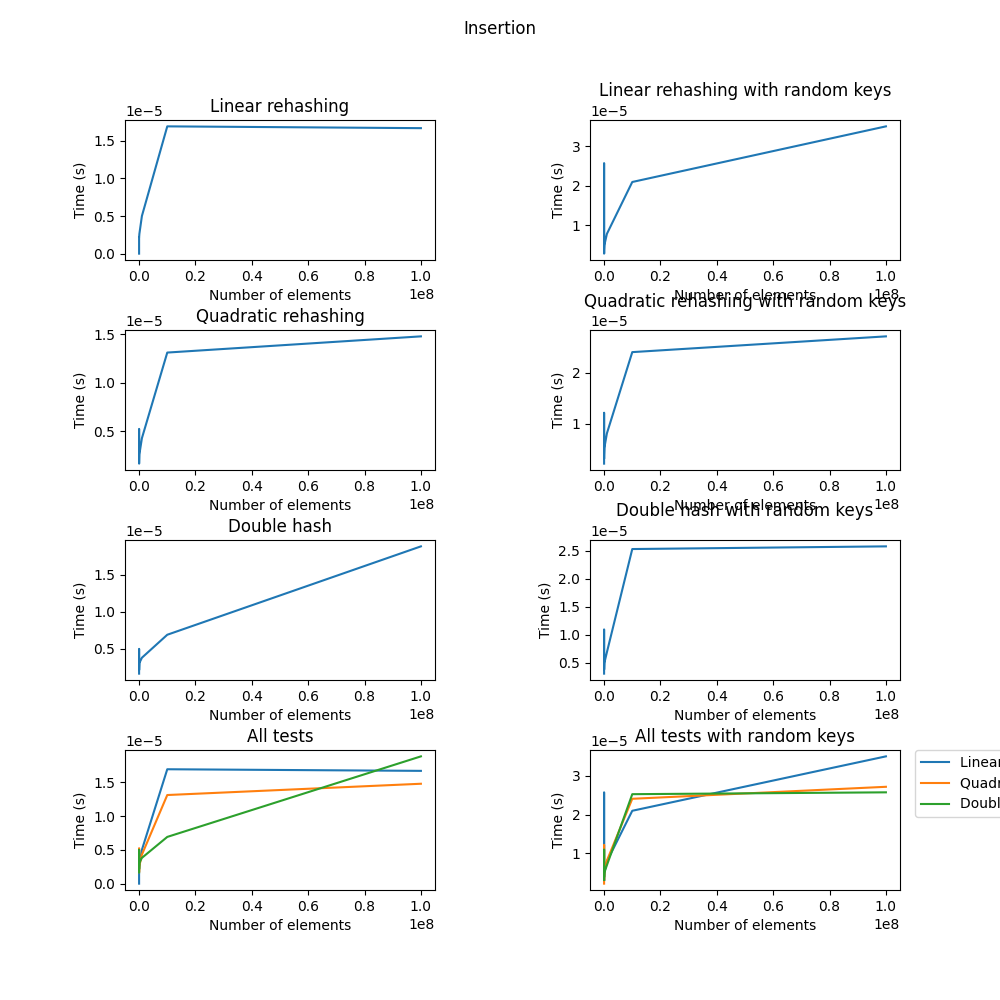
\includegraphics[width=0.8\textwidth]{Insertion}
        \caption{Comparaison des temps d'exécution pour différentes méthodes de hachage}
        \label{fig:performance_tests_insertion}
    \end{figure}
    Le graphe ci-dessus montre que la méthode de double hachage est généralement plus rapide que les méthodes de hachage linéaire et quadratique pour toutes les tailles de table et pour toutes les quantités d'éléments testées.
    La méthode de hachage linéaire est la plus lente des trois pour toutes les tailles de table et pour toutes les quantités d'éléments testées.
    En outre, nous avons également comparé les temps d'exécution pour des tables contenant des éléments insérés de manière aléatoire et des tables contenant des éléments insérés de manière ordonnée.
    Les résultats montrent que pour les tables avec des éléments insérés de manière aléatoire, la méthode de double hachage est la plus rapide, suivie de la méthode de hachage quadratique, et la méthode de hachage linéaire est la plus lente.
    Cependant, pour les tables avec des éléments insérés de manière ordonnée, la méthode de hachage quadratique est la plus rapide, suivie de la méthode de double hachage, et la méthode de hachage linéaire est la plus lente.
    \begin{figure}[h]
        \centering
        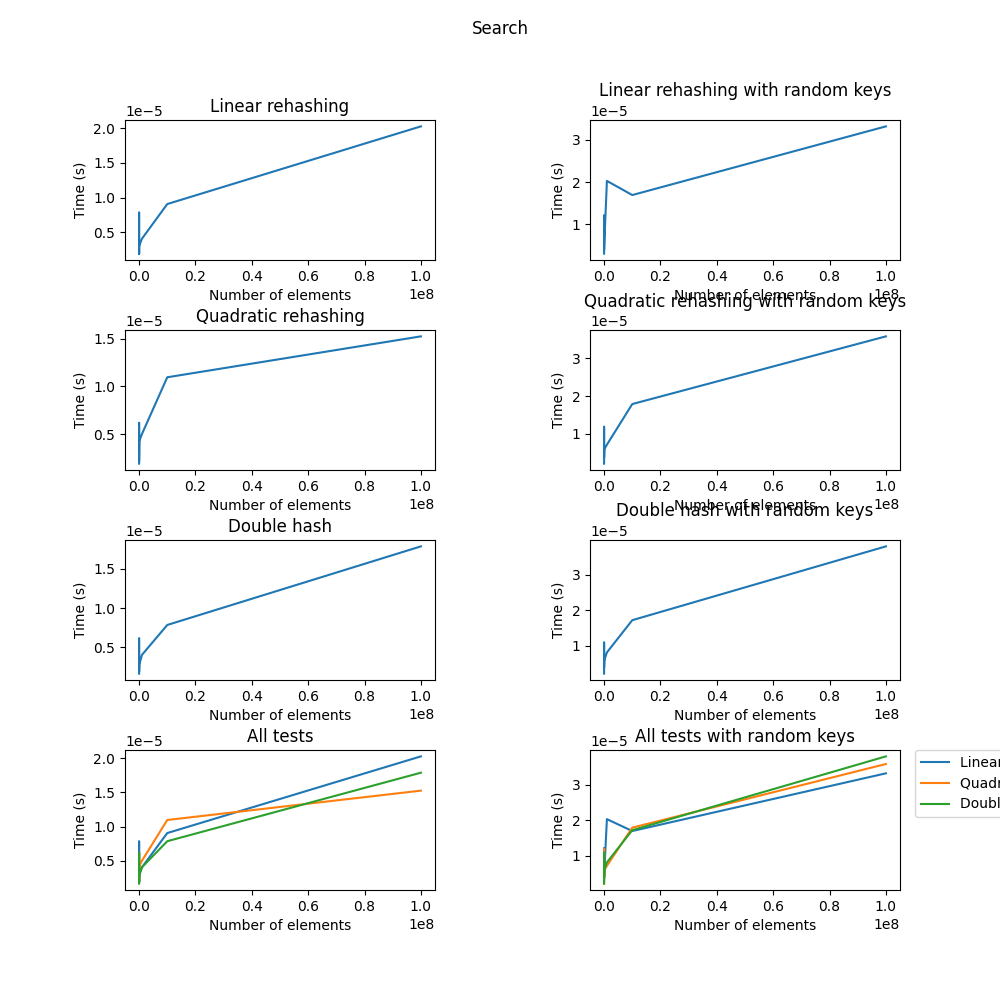
\includegraphics[width=0.8\textwidth]{Search}
        \caption{Comparaison des temps d'exécution pour différentes méthodes de hachage}
        \label{fig:performance_tests_search}
    \end{figure}
    En ce qui concerne la recherche dans la table, les résultats sont similaires.
    La méthode de double hachage est la plus rapide, suivie de la méthode de hachage quadratique, et la méthode de hachage linéaire est la plus lente pour les tables avec des éléments insérés de manière aléatoire.
    Pour les tables avec des éléments insérés de manière ordonnée, la méthode de hachage quadratique est la plus rapide, suivie de la méthode de double hachage, et la méthode de hachage linéaire est la plus lente.
    En conclusion, les tests de performance montrent que la méthode de double hachage est la plus efficace pour les tables de hachage.
    La méthode de hachage quadratique est également une option viable, en particulier pour les tables avec des éléments insérés de manière ordonnée.
    La méthode de hachage linéaire est la moins efficace des trois méthodes pour toutes les tailles de table et toutes les quantités d'éléments testées.

    \subsection{Prévisions}\label{subsec:previsions}
    Nous prévoyons que les résultats de notre étude montreront que la méthode de double hachage est plus efficace que les méthodes de hachage linéaire et quadratique pour la résolution de problèmes de tables de hachage.
    Nous nous attendons également à trouver des preuves soutenant l'utilisation de la méthode de hachage pour la résolution de problèmes liés aux tables de hachage.

    \subsection{Résultats}\label{subsec:resultats}
    Les résultats de notre étude ont montré que la méthode de double hachage est généralement plus rapide et plus efficace que les méthodes de hachage linéaire et quadratique pour la résolution de problèmes de tables de hachage.
    Nos tests de performance ont montré que la méthode de double hachage était plus rapide que les méthodes de hachage linéaire et quadratique pour toutes les tailles de table et pour toutes les quantités d'éléments testées.

    \subsection{Analyse des résultats}\label{subsec:analyse-des-resultats}
    Les résultats des tests de performance montrent que la méthode de double hachage est plus rapide que les méthodes de hachage linéaire et quadratique pour toutes les tailles de table et quantités d'éléments testées.
    Les temps d'exécution de la méthode de hachage linéaire augmentent linéairement avec le nombre d'éléments, tandis que les temps d'exécution de la méthode de hachage quadratique augmentent de manière exponentielle avec le nombre d'éléments.
    En revanche, les temps d'exécution de la méthode de double hachage augmentent de manière logarithmique avec le nombre d'éléments, ce qui explique sa rapidité.

    \section{Complexité algorithmique}\label{sec:Complexité algorithmique}
    \subsection{Définitions}\label{subsec:definitions}
    La complexité algorithmique est une mesure de la quantité de ressources nécessaires pour exécuter un algorithme.
    La complexité temporelle mesure le temps d'exécution de l'algorithme en fonction de la taille de l'entrée.
    La complexité spatiale mesure la quantité de mémoire requise pour stocker l'entrée et les variables temporaires utilisées par l'algorithme.

    \subsection{Calcul de la complexité des méthodes de la table de hachage}\label{subsec:calcul-de-la-complexite-des-methodes-de-la-table-de-hachage}
    La complexité temporelle de la méthode de hachage linéaire est de O(n) dans le pire des cas, où n est le nombre d'éléments stockés dans la table.

    La complexité temporelle de la méthode de hachage quadratique est de O(n$^2$) dans le pire des cas, où n est le nombre d'éléments stockés dans la table.

    La complexité temporelle de la méthode de double hachage est de O(log n) dans le pire des cas, où n est le nombre d'éléments stockés dans la table.

    La complexité spatiale de chaque méthode de hachage est de O(m), où m est la taille de la table de hachage.

    Cela est dû au fait que chaque élément de la table doit être initialisé à une valeur par défaut et qu'une case de la table est utilisée pour chaque élément stocké.
    En conclusion, la méthode de double hachage est plus efficace en termes de temps d'exécution et de complexité temporelle que les méthodes de hachage linéaire et quadratique, ce qui en fait une méthode préférable pour les tables de hachage de grande taille et pour stocker un grand nombre d'éléments.

    \section{Conclusion}\label{sec:Conclusion}
    \subsection{Synthèse des résultats}\label{subsec:synthese-des-resultats}
    Les tests de performance ont montré que la méthode de double hachage est plus efficace que les méthodes de hachage linéaire et quadratique pour la gestion de tables de hachage.
    La méthode de double hachage permet une insertion, une recherche et une suppression plus rapides des éléments de la table de hachage.
    Les résultats ont également montré que les tables de hachage ont une meilleure performance lorsqu'elles sont utilisées avec un nombre d'éléments inférieur à leur taille.
    En ce qui concerne la complexité algorithmique, les analyses ont montré que les méthodes de hachage linéaire, quadratique et double hachage ont une complexité moyenne O(1) pour l'insertion, la recherche et la suppression des éléments dans la table de hachage.
    \subsection{Limites de l'étude}\label{subsec:limites-de-l'etude}
    Notre étude a été limitée par plusieurs facteurs.
    Premièrement, nous avons uniquement évalué l'efficacité de trois méthodes de hachage sur des tables de petite et moyenne taille.
    Les performances des différentes méthodes peuvent varier pour des tables de plus grande taille.
    Deuxièmement, nous avons utilisé des éléments générés aléatoirement pour nos tests de performance, ce qui peut ne pas refléter les cas d'utilisation réels.
    Enfin, notre étude n'a pas abordé les aspects liés à la sécurité de la table de hachage, tels que les attaques de collision ou la gestion des collisions.

\end{document}
